%% abtex2-modelo-trabalho-academico.tex, v-1.9.2 laurocesar
%% Copyright 2012-2014 by abnTeX2 group at http://abntex2.googlecode.com/ 
%%
%% This work may be distributed and/or modified under the
%% conditions of the LaTeX Project Public License, either version 1.3
%% of this license or (at your option) any later version.
%% The latest version of this license is in
%%   http://www.latex-project.org/lppl.txt
%% and version 1.3 or later is part of all distributions of LaTeX
%% version 2005/12/01 or later.
%%
%% This work has the LPPL maintenance status `maintained'.
%% 
%% The Current Maintainer of this work is the abnTeX2 team, led
%% by Lauro César Araujo. Further information are available on 
%% http://abntex2.googlecode.com/
%%
%% This work consists of the files abntex2-modelo-trabalho-academico.tex,
%% abntex2-modelo-include-comandos and abntex2-modelo-references.bib
%%

% ------------------------------------------------------------------------
% ------------------------------------------------------------------------
% abnTeX2: Modelo de Trabalho Academico (tese de doutorado, dissertacao de
% mestrado e trabalhos monograficos em geral) em conformidade com 
% ABNT NBR 14724:2011: Informacao e documentacao - Trabalhos academicos -
% Apresentacao
% ------------------------------------------------------------------------
% ------------------------------------------------------------------------


\documentclass[
        % -- opções da classe memoir --
        12pt,                           % tamanho da fonte
        openright,                      % capítulos começam em pág ímpar (insere página vazia caso preciso)
        twoside,                        % para impressão em verso e anverso. Oposto a oneside
        a4paper,                        % tamanho do papel. 
        % -- opções da classe abntex2 --
        %chapter=TITLE,         % títulos de capítulos convertidos em letras maiúsculas
        %section=TITLE,         % títulos de seções convertidos em letras maiúsculas
        %subsection=TITLE,      % títulos de subseções convertidos em letras maiúsculas
        %subsubsection=TITLE,% títulos de subsubseções convertidos em letras maiúsculas
        % -- opções do pacote babel --
        english,                        % idioma adicional para hifenização
        french,                         % idioma adicional para hifenização
        spanish,                        % idioma adicional para hifenização
        brazil                          % o último idioma é o principal do documento
        ]{abntex2}

% ---
% Pacotes básicos 
% ---
\usepackage{lmodern}                    % Usa a fonte Latin Modern                      
\usepackage[T1]{fontenc}                % Selecao de codigos de fonte.
\usepackage[utf8]{inputenc}             % Codificacao do documento (conversão automática dos acentos)
\usepackage{lastpage}                   % Usado pela Ficha catalográfica
\usepackage{indentfirst}                % Indenta o primeiro parágrafo de cada seção.
\usepackage{color}                      % Controle das cores
\usepackage{graphicx}                   % Inclusão de gráficos
\usepackage{microtype}                  % para melhorias de justificação
\definecolor{blue}{RGB}{41,5,195}
%\emergencystretch=1.5em
%\tolerance=270
% ---

% ---
% Pacotes de citações
% ---
\usepackage[brazilian,hyperpageref]{backref}     % Paginas com as citações na bibl
\usepackage[alf]{abntex2cite}                    % Citações padrão ABNT
\usepackage{lmodern}                             % Usa a fonte Latin Modern                      
\usepackage[T1]{fontenc}                         % Selecao de codigos de fonte.
\usepackage[utf8]{inputenc}                      % Codificacao do documento (conversão automática dos acentos)
\usepackage{lastpage}                            % Usado pela Ficha catalográfica
\usepackage{indentfirst}                         % Indenta o primeiro parágrafo de cada seção.
\usepackage{color}                               % Controle das cores
\usepackage{microtype}                           % para melhorias de justificação
\usepackage[section]{placeins}

% --- 
% CONFIGURAÇÕES DE PACOTES
% --- 

% ---
% Configurações do pacote backref
% Usado sem a opção hyperpageref de backref
\renewcommand{\backrefpagesname}{Citado na(s) página(s):~}
% Texto padrão antes do número das páginas
\renewcommand{\backref}{}
% Define os textos da citação
\renewcommand*{\backrefalt}[4]{
        \ifcase #1 %
                Nenhuma citação no texto.%
        \or
                Citado na página #2.%
        \else
                Citado #1 vezes nas páginas #2.%
        \fi}%

\usepackage{amsmath, amssymb, amscd, amsthm, amsfonts}
\usepackage{physics}
\usepackage{bm}
\usepackage{graphicx}
\usepackage{hyperref}

\usepackage{tikz}
\usepackage{pgfplots}
\usepackage{tabto}
\usepackage[siunitx]{circuitikz}
\usetikzlibrary{patterns, arrows, calc, decorations}
\usetikzlibrary{decorations.markings}
\usetikzlibrary{decorations.text}
\usepackage{hyperref}
\hypersetup{
  colorlinks=true,linkcolor=blue,urlcolor=cyan
}
% \usepackage[portuguese]{babel} % Corrige linguaagem
\usepackage{svg}

\title{Eletro\'im\~as e suas aplicaç\~oes}
\author{Juan Vasconcelos, Matrícula: 201907140019 \and Jo\~ao Pedro Albuquerque, Matrícula: 201907140017 \and Jo\~ao Paulo de Andrade, Matrícula: 201907140009 \and Thiago Toni, Matrícula: 201907140061}
\date{}


\instituicao{%
  Universidade Federal do Pará
  \par
  Faculdade de Engenharia Elétrica e Biomédica
  }
\tipotrabalho{Trabalho Acadêmico}

\makeatletter
\hypersetup{
        %pagebackref=true,
                pdftitle={\@title}, 
                pdfauthor={\@author},
                pdfsubject={\imprimirpreambulo},
                pdfcreator={LaTeX with abnTeX2},
                pdfkeywords={abnt}{latex}{abntex}{abntex2}{trabalho acadêmico}, 
                colorlinks=true,                % false: boxed links; true: colored links
                linkcolor=blue,                 % color of internal links
                citecolor=blue,                 % color of links to bibliography
                filecolor=magenta,                      % color of file links
                urlcolor=blue,
                bookmarksdepth=4
}
\makeatother

\begin{document}

\frenchspacing 

\imprimircapa

\imprimirfolhaderosto*

\setlength{\absparsep}{18pt} % ajusta o espaçamento dos parágrafos do resumo
\begin{resumo}
  Este trabalho condensa contexto histórico, embasamento e modelagem matemática e
  aplicações do Eletroímã. O texto se inicia com uma apresentação do concebimento
  do eletroímã e mostrando algumas aplicações de forma rasa, aprofunda na modelagem
  matemática e elabora nas aplicações.
\end{resumo}


% ---
% inserir lista de ilustrações
% ---
\pdfbookmark[0]{\listfigurename}{lof}
\listoffigures*
\cleardoublepage
% ---

% ---
% inserir lista de tabelas
% ---
\pdfbookmark[0]{\listtablename}{lot}
\listoftables*
\cleardoublepage
% ---

% ---
% inserir o sumario
% ---
\pdfbookmark[0]{\contentsname}{toc}
\tableofcontents*
\cleardoublepage
% ---

% \tableofcontents

%% Introdução

\part{Introdução}
\chapter[Contexto Histórico]{Contexto Histórico}

\section{A Invenção do Eletroímã}\label{chap:introdução:sec:invenção}
Eletroímãs estão presentes desde 1824 com a invenção de William Sturgeon após
a descorberta de Hans Christian Ørsted em 1820 onde descreve que a corrente elétrica
de um fio deflete uma bússola. Sua invenção, presente na
figura~\ref{fig:chap:introdução:1}, consistia de um pedaço de ferro maciço em formato
de ferradura de cavalo envolvido por um condutor. O grande destaque do dispositivo
era a proporção de seu peso próprio com o peso que conseguia levantar, pesando apenas
200 gramas o aparelho sustentava cargas de até aproximadamente 4 quilos.

\begin{figure}[!htp]
  \centering
  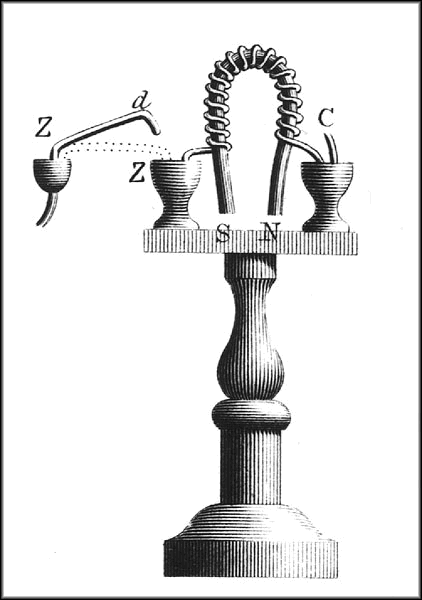
\includegraphics[width=0.2\columnwidth]{Sturgeon_electromagnet.png}
  \label{fig:chap:introdução:1}
  \caption{Eletroímã de Sturgeon \cite{web:wikipedia:electromagnet}}
\end{figure}
O dispositivo possuía a desvantagem de não ser muito eficiente, pois o mesmo utilizava
fios com isolamento pouco flexível, que limitou o número de voltas envolvendo o
pedaço de ferro. Seu princípio de funcionamento serviu para o decodificador de telégrafo. Inventado
em 1850 por Alfred Vail, o dispositivo move a ponta de uma haste de metal para
martelar uma superfície e produzir um sinal sonoro. Era usual a transmissão das
mensagens em código morse pelo meio.
\begin{figure}[!htp]
  \centering
  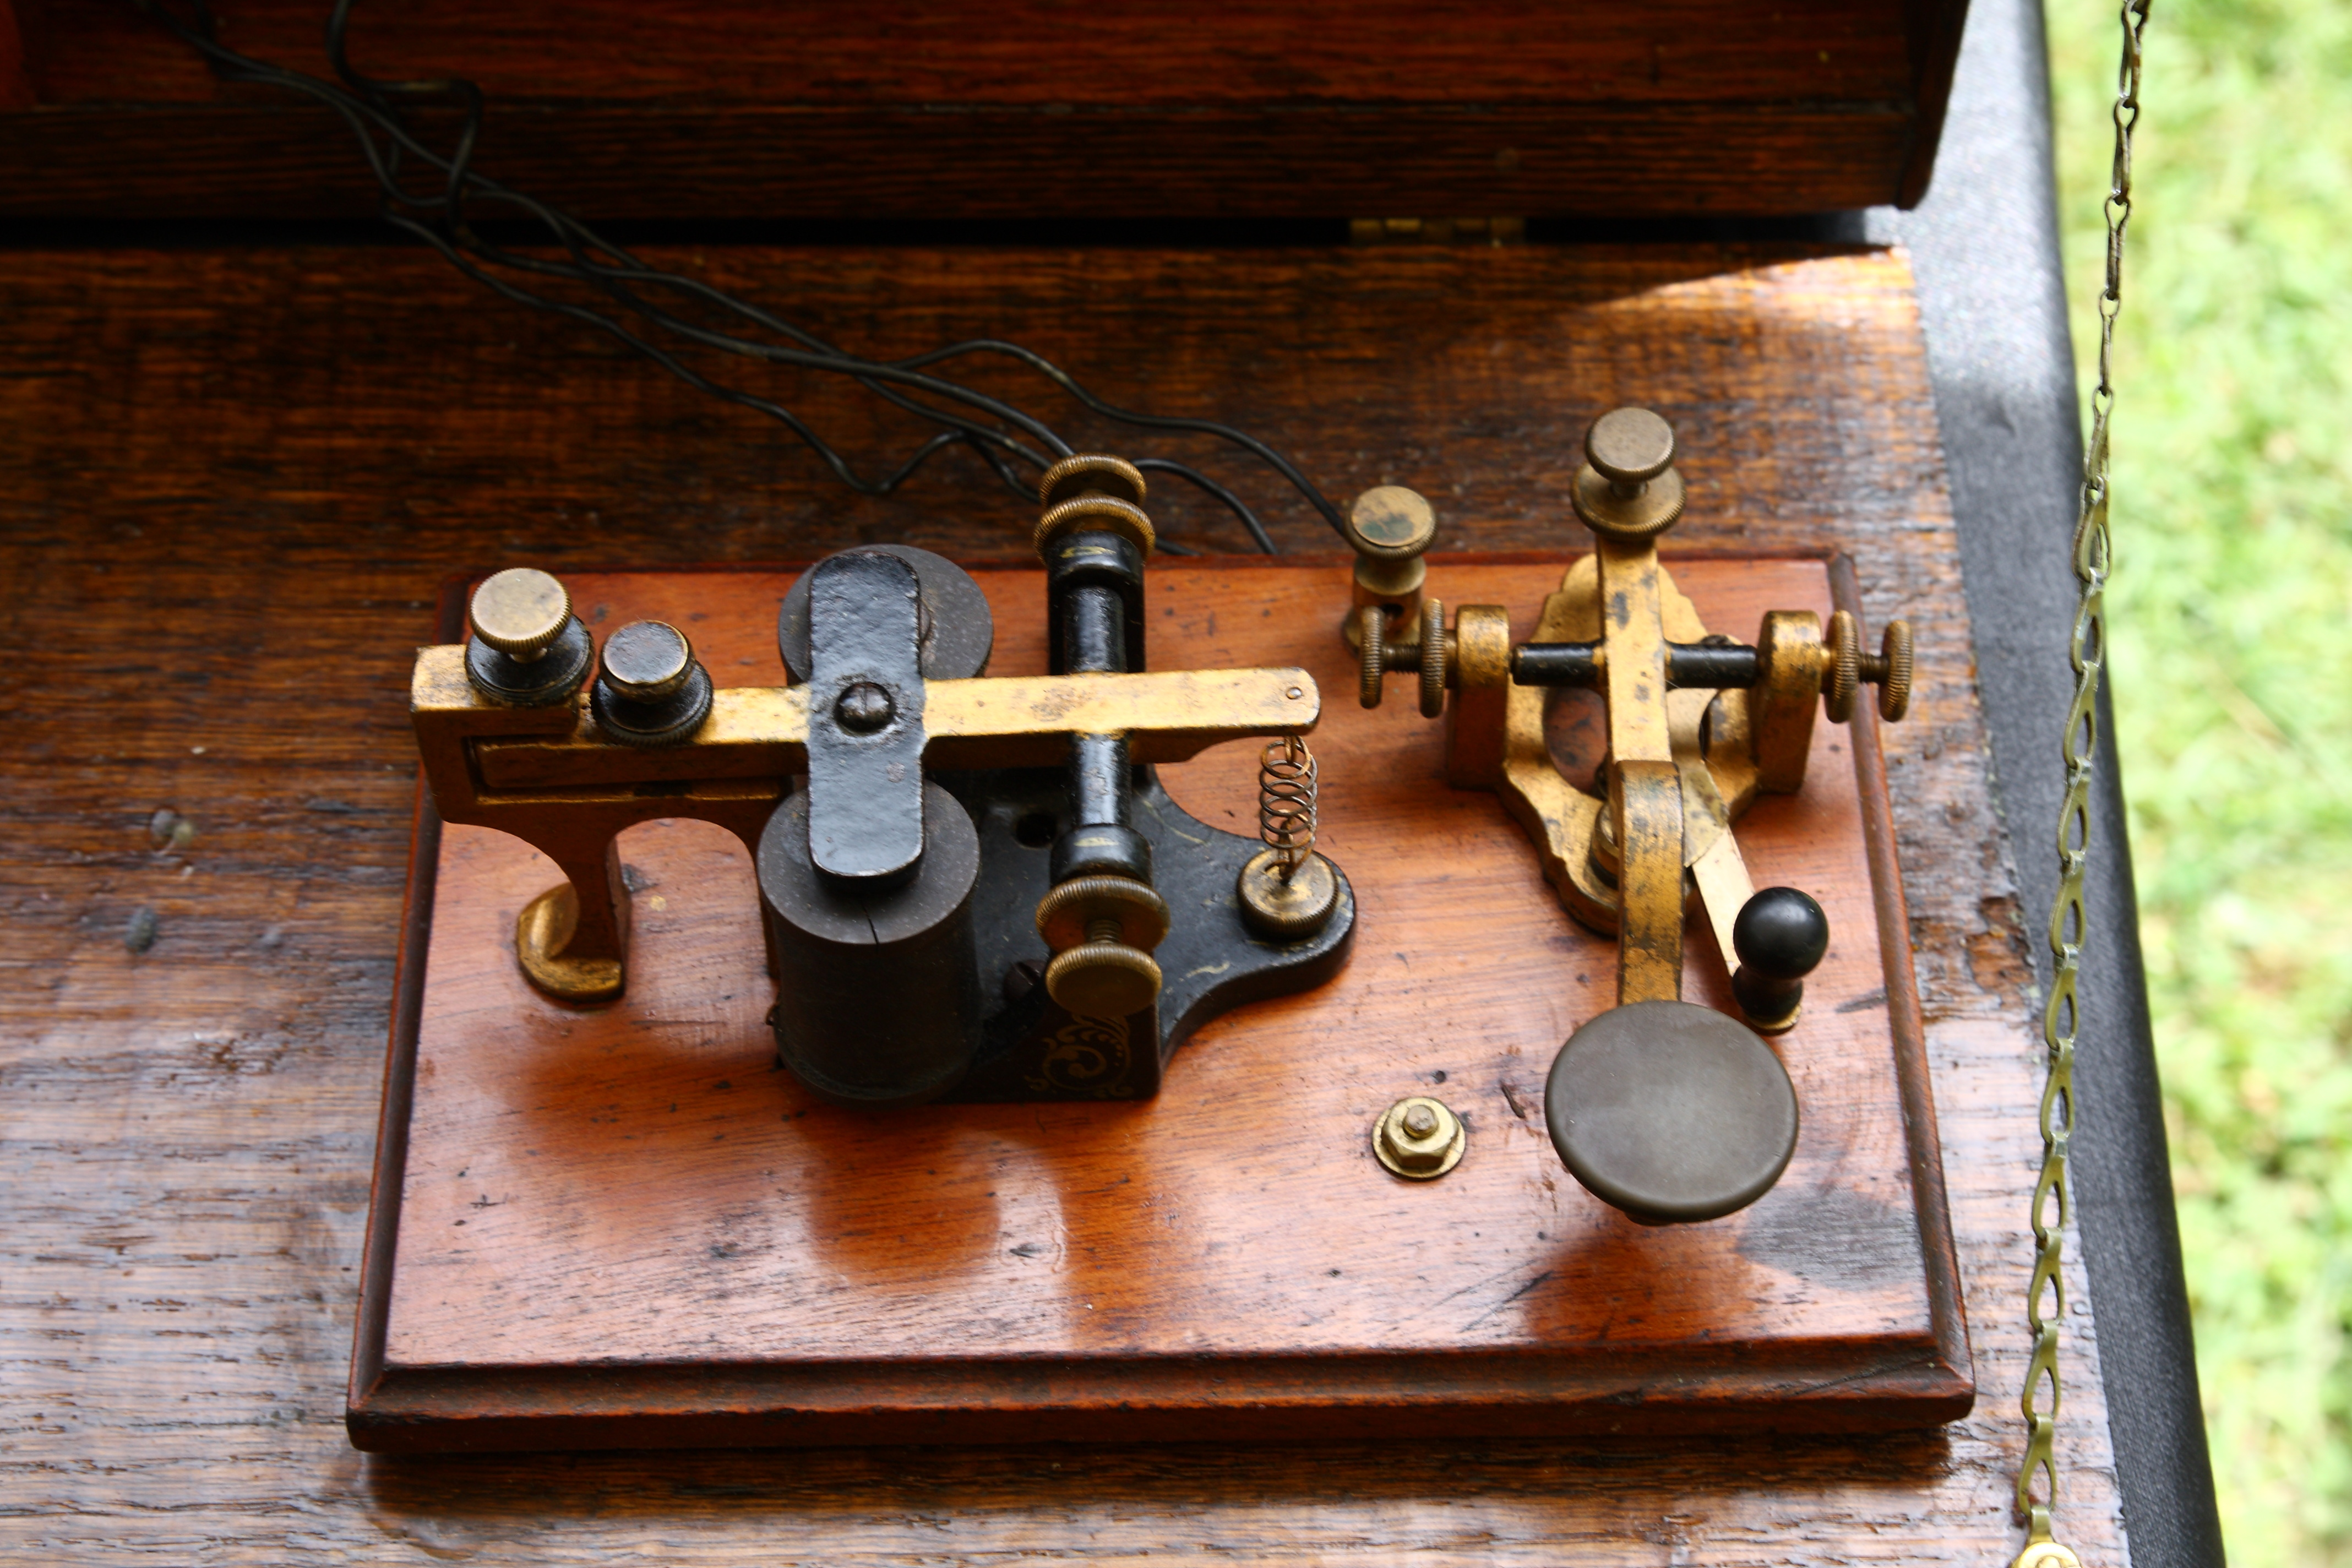
\includegraphics[width=0.3\columnwidth]{Wallace_Study-Telegraph.jpg}
  \label{fig:chap:introdução:2}
  \caption{Aparelho de telégrafo \cite{web:wikipedia:telegraph}}
\end{figure}

\section{Aplicações} \label{chap:introducao:sec:aplicações}
O eletroímã ganhou várias aplicações conforme seu funcionamento foi explorado, o
eletroímã foi empregado em mais e mais dispositivos. Neste trabalho damos enfoque
às seguintes aplicações:
\begin{itemize}
  \item Motores
  \item Transformadores
  \item Relés
  \item Levitação Magnética
\end{itemize}

%% Desenvolvimento

\part{Desenvolvimento}
\chapter[Embasamento Matemático]{Embasamento Matemático}\label{chap:embasamento}
\section{Indução Magnética e a Lei de Ampère}
O princípio de funcionamento de eletroímãs advem da Lei de Ampère:
\begin{gather}
  \underbrace{ \oint_{\partial \Sigma} \bm{B} \cdot \: d{\bm{l}} }_\text{ campo magnético } = \mu_0 \left( \underbrace{ \iint_{\Sigma} \bm{J} \cdot \: d{\bm{S}} }_\text{corrente} + \underbrace{ \varepsilon \dfrac{d}{dt} \iint_{\Sigma} \bm{E} \: d{\bm{S}} }_\text{componente variante no tempo}  \right)
\end{gather}
ou igualmente em sua forma diferencial:
\begin{gather}
  \underbrace{\nabla \times \bm{B}}_\text{campo magnético} = \mu_0 \left( \underbrace{\bm{J}}_\text{corrente} + \underbrace{\varepsilon \dfrac{\partial \bm{E}}{\partial t}}_\text{componente variante no tempo} \right) 
\end{gather}
\begin{figure}[!htp]
  \centering
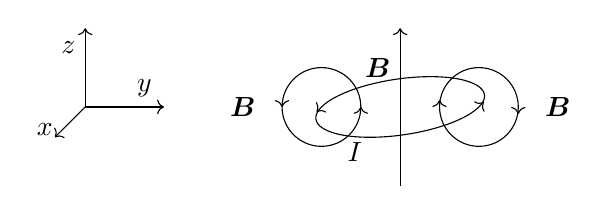
\begin{tikzpicture}
  % anel com corrente
  \draw[
    decoration={markings, mark=at position 0 with {\arrow{<}}},
    decoration={markings, mark=at position 0.5 with {\arrow{<}}},
    postaction={decorate}
    ] (0,0,0) [y={(0,0,1)}] circle (1) node[above left] {};
  \node at (0,1.5,0) [y={(0,0,1)}] {$I$};
  
  % Campo magnético
  \draw[
    decoration={markings, mark=at position 0 with {\arrow{<}}},
    decoration={markings, mark=at position 0.5 with {\arrow{<}}},
    postaction={decorate}
    ] (1,0,0) [y={(0,1,0)}] circle (0.5);
  \node at (2,0,0) [y={(0,1,0)}] {$\bm{B}$};
  \draw[
    decoration={markings, mark=at position 0 with {\arrow{>}}},
    decoration={markings, mark=at position 0.5 with {\arrow{>}}},
    postaction={decorate}
    ] (-1,0,0) [y={(0,1,0)}] circle(0.5);
  \node at (-2,0,0) [y={(0,1,0)}] {$\bm{B}$};
  \draw[->] (0,-1,0) [y={(0,1,0)}] -- ++(0,2,0) node[left, near end]{$\bm{B}$};


  \draw[->] (-4,0,0) [y={(0,1,0)}] -- ++(0,1,0) node[left, near end]{$z$};
  \draw[->] (-4,0,0) [y={(0,0,1)}] -- ++(0,1,0) node[left, near end]{$x$};
  \draw[->] (-4,0,0) [y={(0,0,1)}] -- ++(1,0,0) node[above, near end]{$y$};
\end{tikzpicture}
\label{fig:chap:embasamento:1}
\caption{Campo magnético atravessando um anel com corrente anti-horária (Autores)}
\end{figure}

Ignorando por hora a componente variante no tempo, podemos nos focar no resultado
interessante para máquinas assíncronas: corrente elétrica em um condutor gera um
campo magnético, como ilustrado na figura~\ref{fig:chap:embasamento:1}. Enrolando
um condutor em forma helicoidal (um solenóide), que equivale a alinhar anéis em
sequência, teremos uma amplificação do campo, devido à contribuição de cada porção
de corrente no condutor, como exposto na figura~\ref{fig:chap:embasamento:2}.

\begin{figure}[!htp]
  \centering
  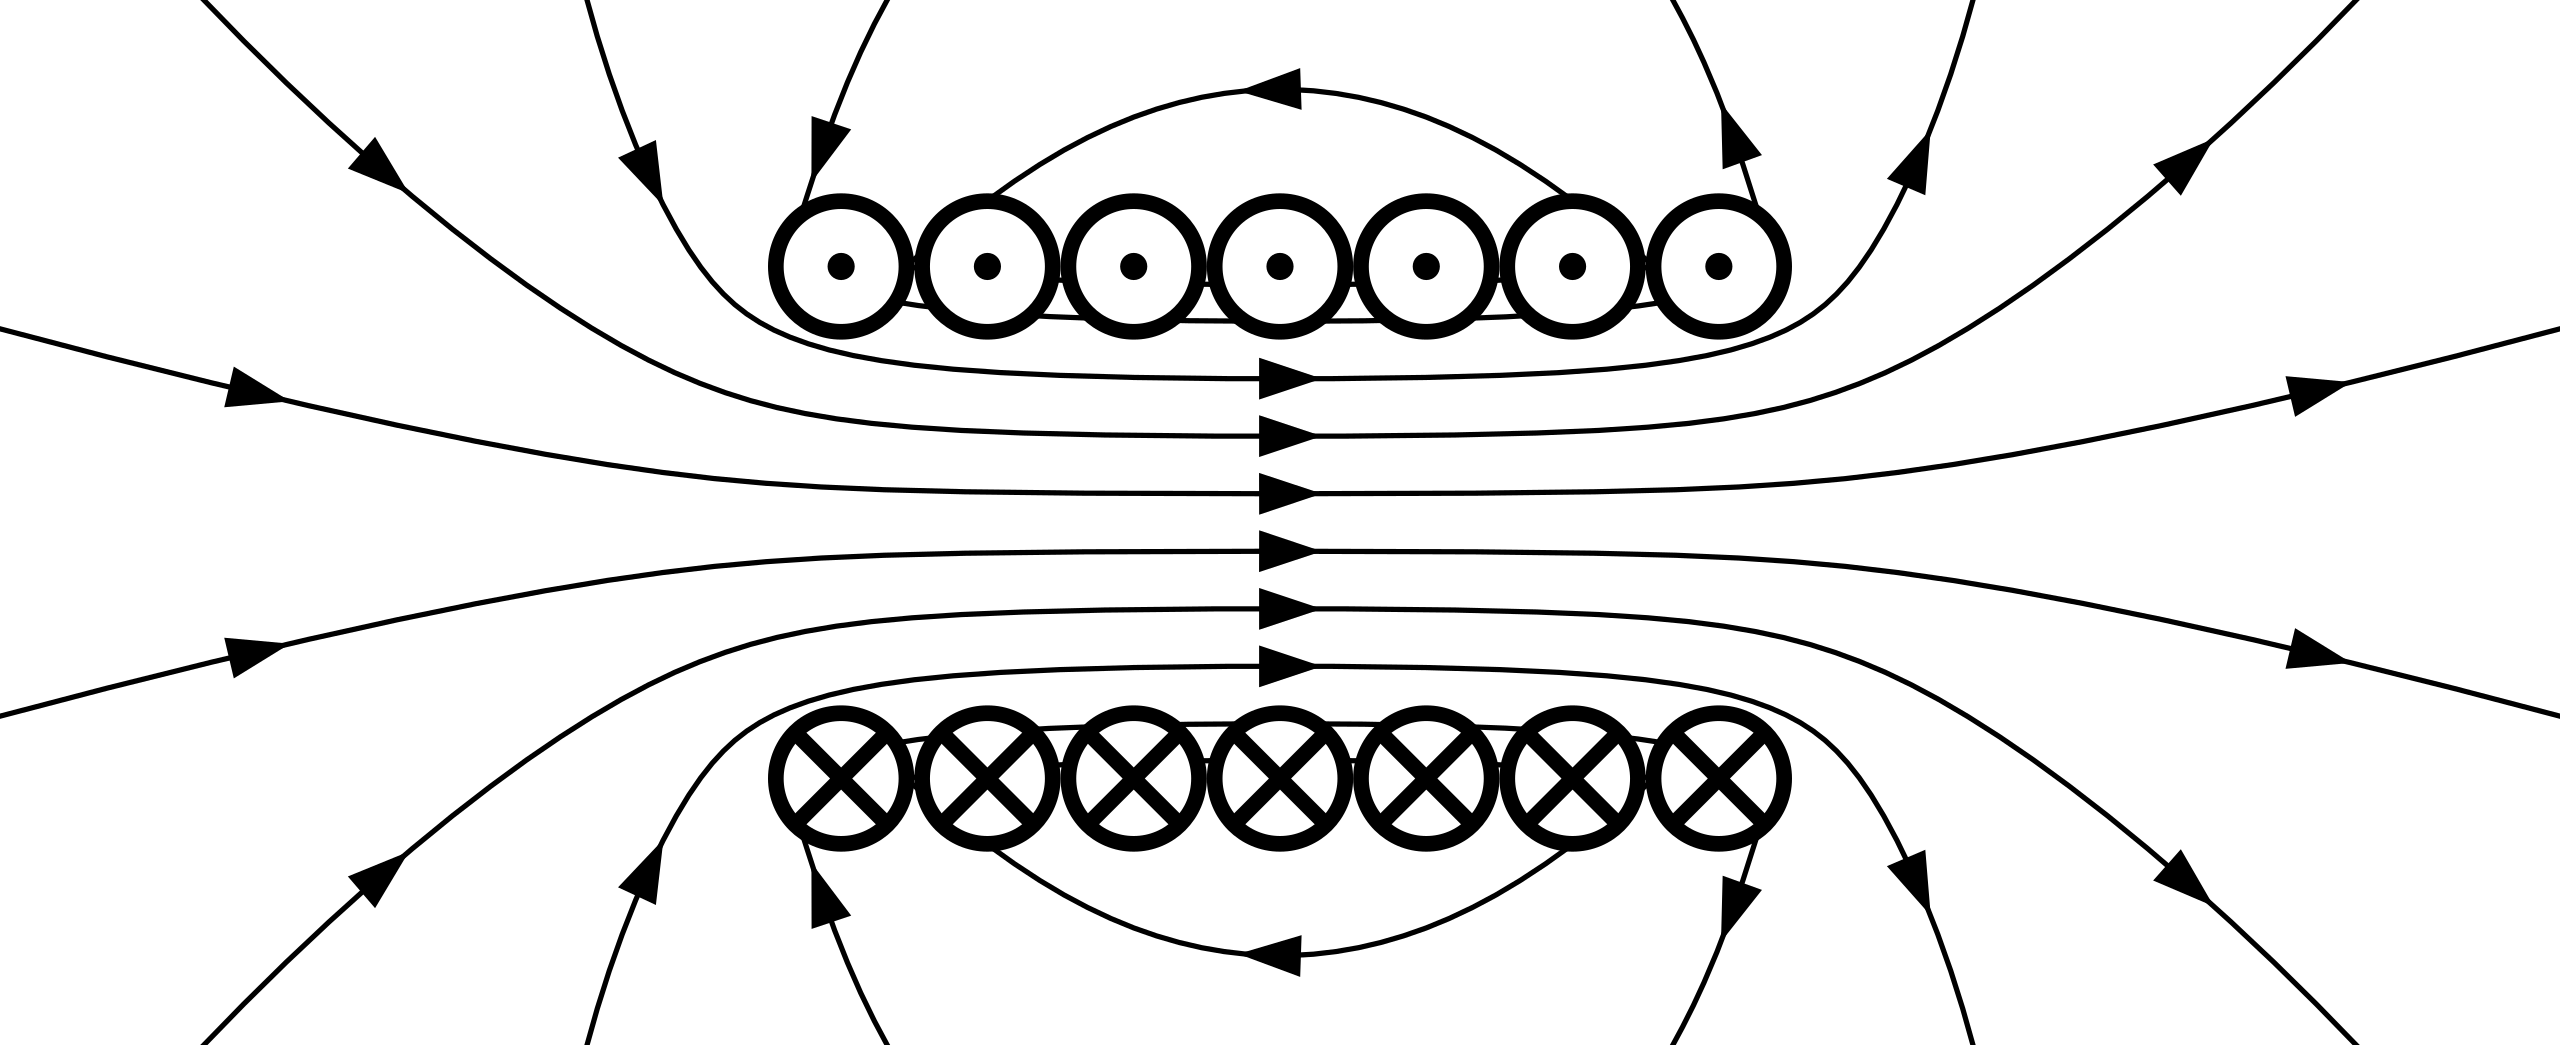
\includegraphics[width=0.5\columnwidth]{2560px-VFPt_Solenoid_correct2.svg.png}
  \label{fig:chap:embasamento:2}
  \caption{Campo magnético dentro de um solenóide}
\end{figure}

\section{Magnetismo e Ferromagnetismo}
A organização e disposição da estrutura e substância afetam o quanto um material
é suscetível à passagem de campos magnéticos. Seguindo a descrição proposta em
\cite{book:balanis}, podemos analisar as propriedades macroscópicas de materiais
em função de sua organização microscópica.

Sem se ater à descrições envolvendo mecânica quântica, afinal tal precisão se mostra
desnecessária para as descrições aqui feitas, podemos nos utilizar de um modelo
atômico simples, com elétrons em órbitas circulares em volta de um núcleo positivo
(figura~\ref{fig:chap:embasamento:3}). Podemos então enxergar um material como uma
disposição de pequenos dipolos magnéticos com momentos de dipolo magnético $\dd \bm{m}_i$
dado por:

\begin{gather}
  \dd{\bm{m}_i} = I_i \dd \bm{s}_i = \bm{\hat{n}}I_i \dd s_i \quad (\text{A}-\text{m}^2)
\end{gather}

\begin{figure}[!htp]
  \centering
  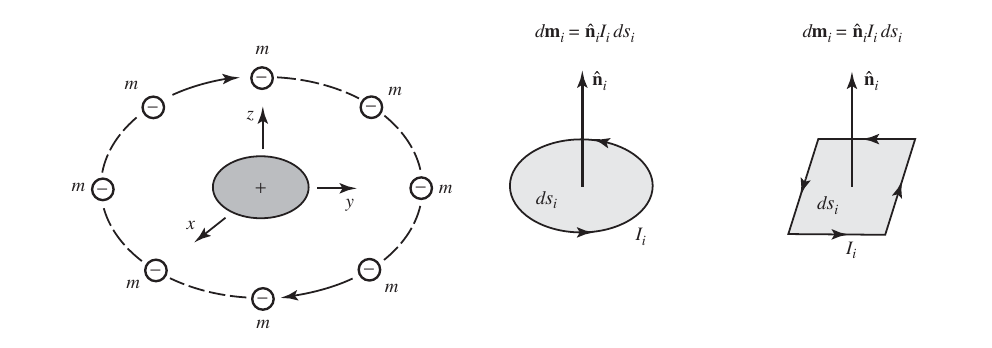
\includegraphics[width=0.9\columnwidth]{balanis3.png}
  \label{fig:chap:embasamento:3}
  \caption{Modelo atômico empregado e ciclos equivalentes \cite{book:balanis}}
\end{figure}

Podemos então somar as contribuições dos momentos de cada dipolo para átomos com
múltiplos elétrons em órbita tendo a razão do número de elétrons por unidade de
volume $N_m$ em uma porção de volume $\Delta v$:
\begin{gather}
\bm{m}_t = \sum_{i = 1}^{N_m \Delta v}{\dd{\bm{m}_i}}
\end{gather}
E definir o vetor de polarização magnética (magnetização) $\bm{M}$ como:
\begin{gather}
  \bm{M} = \underset{\Delta v \to 0}{\lim} \left[ \dfrac{1}{\Delta v}\bm{m}_t \right] = 
  \underset{\Delta v \to 0}{\lim} \left[ \dfrac{1}{\Delta v} \sum_{i = 1}^{N_m \Delta v}{\dd{\bm{m}_i}} \right]
  \quad (\text{A}/\text{m}^2)
\end{gather}
Assumindo que cada caminho tenha um momento médio:
\begin{gather}
  \dd \bm{m}_i = \dd \bm{m}_{av} = \bm{\hat{n}}(I \dd s)_{av} \to
  \bm{M} = N_m \dd \bm{m}_{av} = \bm{\hat{n}} n_m (i \dd s)_{av}
\end{gather}

Podemos então visualizar o comportamento do material antes e após a aplicação de um
vetor densidade de fluxo magnético médio $\bm{B}_a$ na figura~\ref{fig:chap:embasamento:4},
com os dipolos se alinhando à direção do campo.

\begin{figure}[!htp]
  \centering
  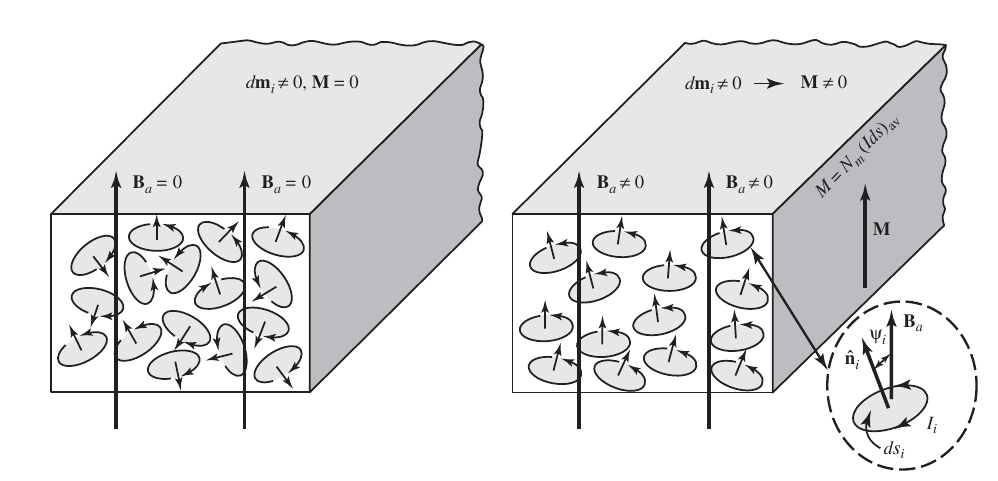
\includegraphics[width=0.9\columnwidth]{balanis2.png}
  \label{fig:chap:embasamento:4}
  \caption{Dipolos magnéticos se alinhando na presença de um campo \cite{book:balanis}}
\end{figure}

Podemos elaborar na ilustração com outra simplificação, utilizando um bloco de material
magnético, Fazendo com que neste bloco tenhamos as contribuições do vetor de magnetização
no vetor densidade de fluxo (figura~\ref{fig:chap:embasamento:5}):
\begin{gather}
  \bm{B} = \mu_0 (\bm{H}_a + \bm{M})
\end{gather}

\begin{figure}[!htp]
  \centering
  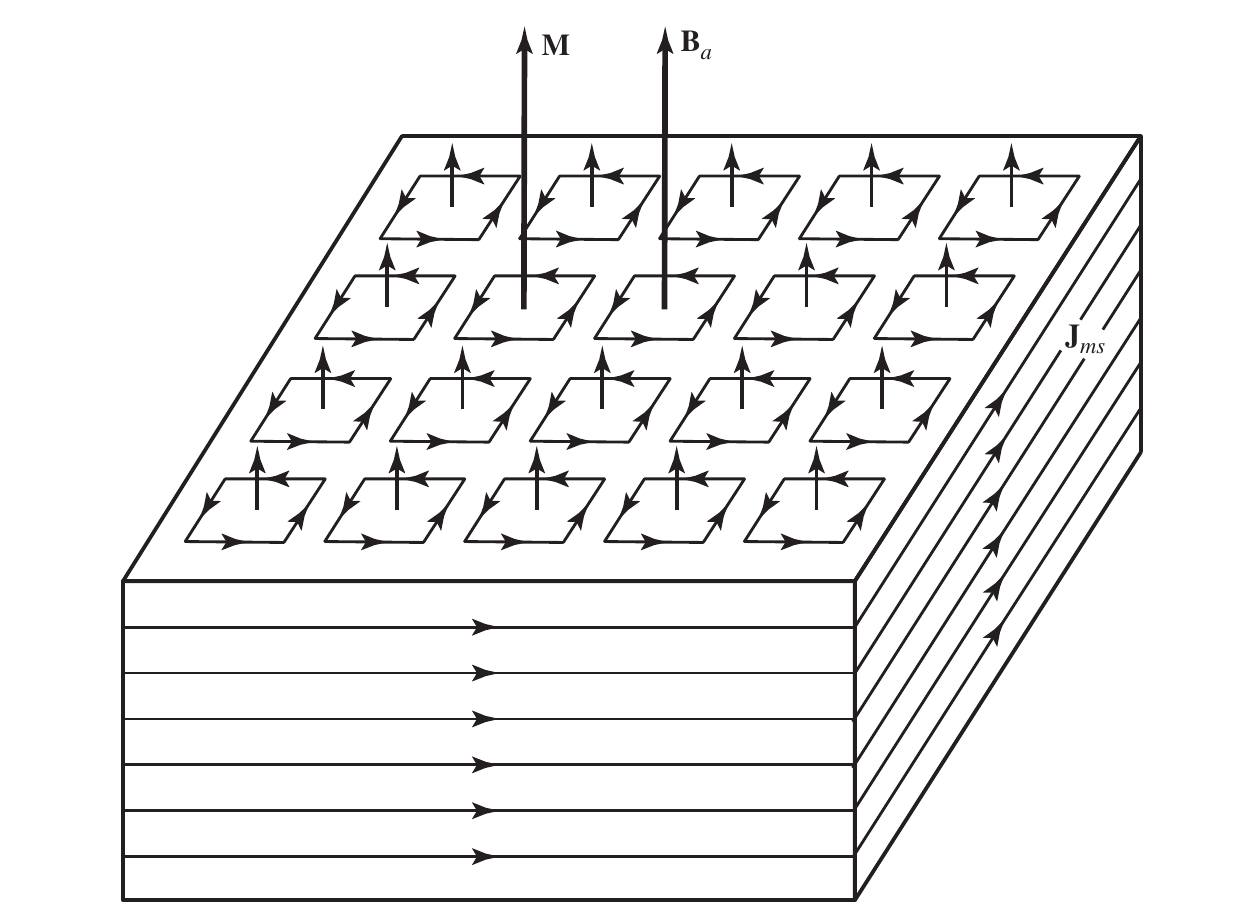
\includegraphics[width=0.7\columnwidth]{balanis.png}
  \label{fig:chap:embasamento:5}
  \caption{Vetores Campo Magnético e de Magnetização em um bloco \cite{book:balanis}}
\end{figure}

Com $\bm{H}_a$ sendo o vetor intensidade de campo magnético médio. Podemos então
escrever:
\begin{gather}
  \bm{B} = \mu_s \bm{H}_a \\
  \bm{M} = \chi_m \bm{H}_a
\end{gather}
Com $\mu_s(H/m)$ sendo a permissividade magnética do meio e $\chi_m(\text{adimensional})$
a susceptibilidade magnética. Assim:

\begin{gather}
  \bm{B} = \mu_0 (\bm{H}_a + \chi_m \bm{H}_a) = \mu_0(1 + \chi_m) \bm{H}_a = \mu_s \bm{H}_a\\
  \mu_s = \mu_0 (1 + \chi_m)
\end{gather}

E temos enfim a definição de permissividade magnética relativa:
\begin{gather}
  \mu_{sr} = \dfrac{\mu_s}{\mu_0} = 1 + \chi_m
\end{gather}

Podemos então prever o comportamento de um material por meio de sua permissividade
magnética relativa, quanto maior sua permissividade, mais suscetível ele será à alinhar
seus dipolos magnéticos a um campo externo aplicado no material. Desse ponto de vista
temos comportamentos diversos de materiais, estas que darão uma denominação ao material
de: diamagnético, não-magnético, ferromagnético, paramagnético,... em conformidade à
sua permissividade. A seguir temos uma tabela com os valores de permissividade de alguns
materiais e sua denominação:

\begin{table}[htpb]
  \centering
  \caption{Valores de $\mu_{sr}$ para alguns materiais \cite{book:balanis}}
  \label{tab:chap1:sec2:mu_values}
  \begin{tabular}{c c c}
    \hline
    Material & Classificação & Permissividade Relativa $\mu_{sr}$\\
    \hline
    Bismute & Diamagnético & 0,999834\\
    Prata & Diamagnético & 0,99998\\
    Chumbo & Diamagnético & 0,999983\\
    Cobre & Diamagnético & 0,999991\\
    Vácuo & Não-Magnético & 1,0\\
    Ar & Paramagnético & 1,0000004\\
    Alumínio & Paramagnético & 1,00002\\
    Cobalto & Ferromagnético & 250\\
    Alumínio & Ferromagnético & 600\\
    Ferro & Ferromagnético & 7000\\
    Ferro Purificado & Ferromagnético & 200.000\\
    \hline
  \end{tabular}
\end{table}

Para nosso trabalho, os materiais ferromagnéticos são os mais interessantes, nome
indicando que se comportam similarmente ao ferro. Estes materiais possuem seus dipolos
desordenados na ausência de campo magnético, porém ao serem excitados seus dipolos se
alinham com pouca resistência, se mostrando um meio propício para a propagação desses
campos. Este comportamento é extremamente interessante, pois, combinada com a indução
pela lei de ampère, podemos inserir campos magnéticos controlados por meio de um
solenoide em um material ferromagnético e utilizá-los para direcionar o campo
em um caminho conveniente sem grande dissipação (figura~\ref{fig:chap:embasamento:6}).

\begin{figure}[!htp]
  \centering
  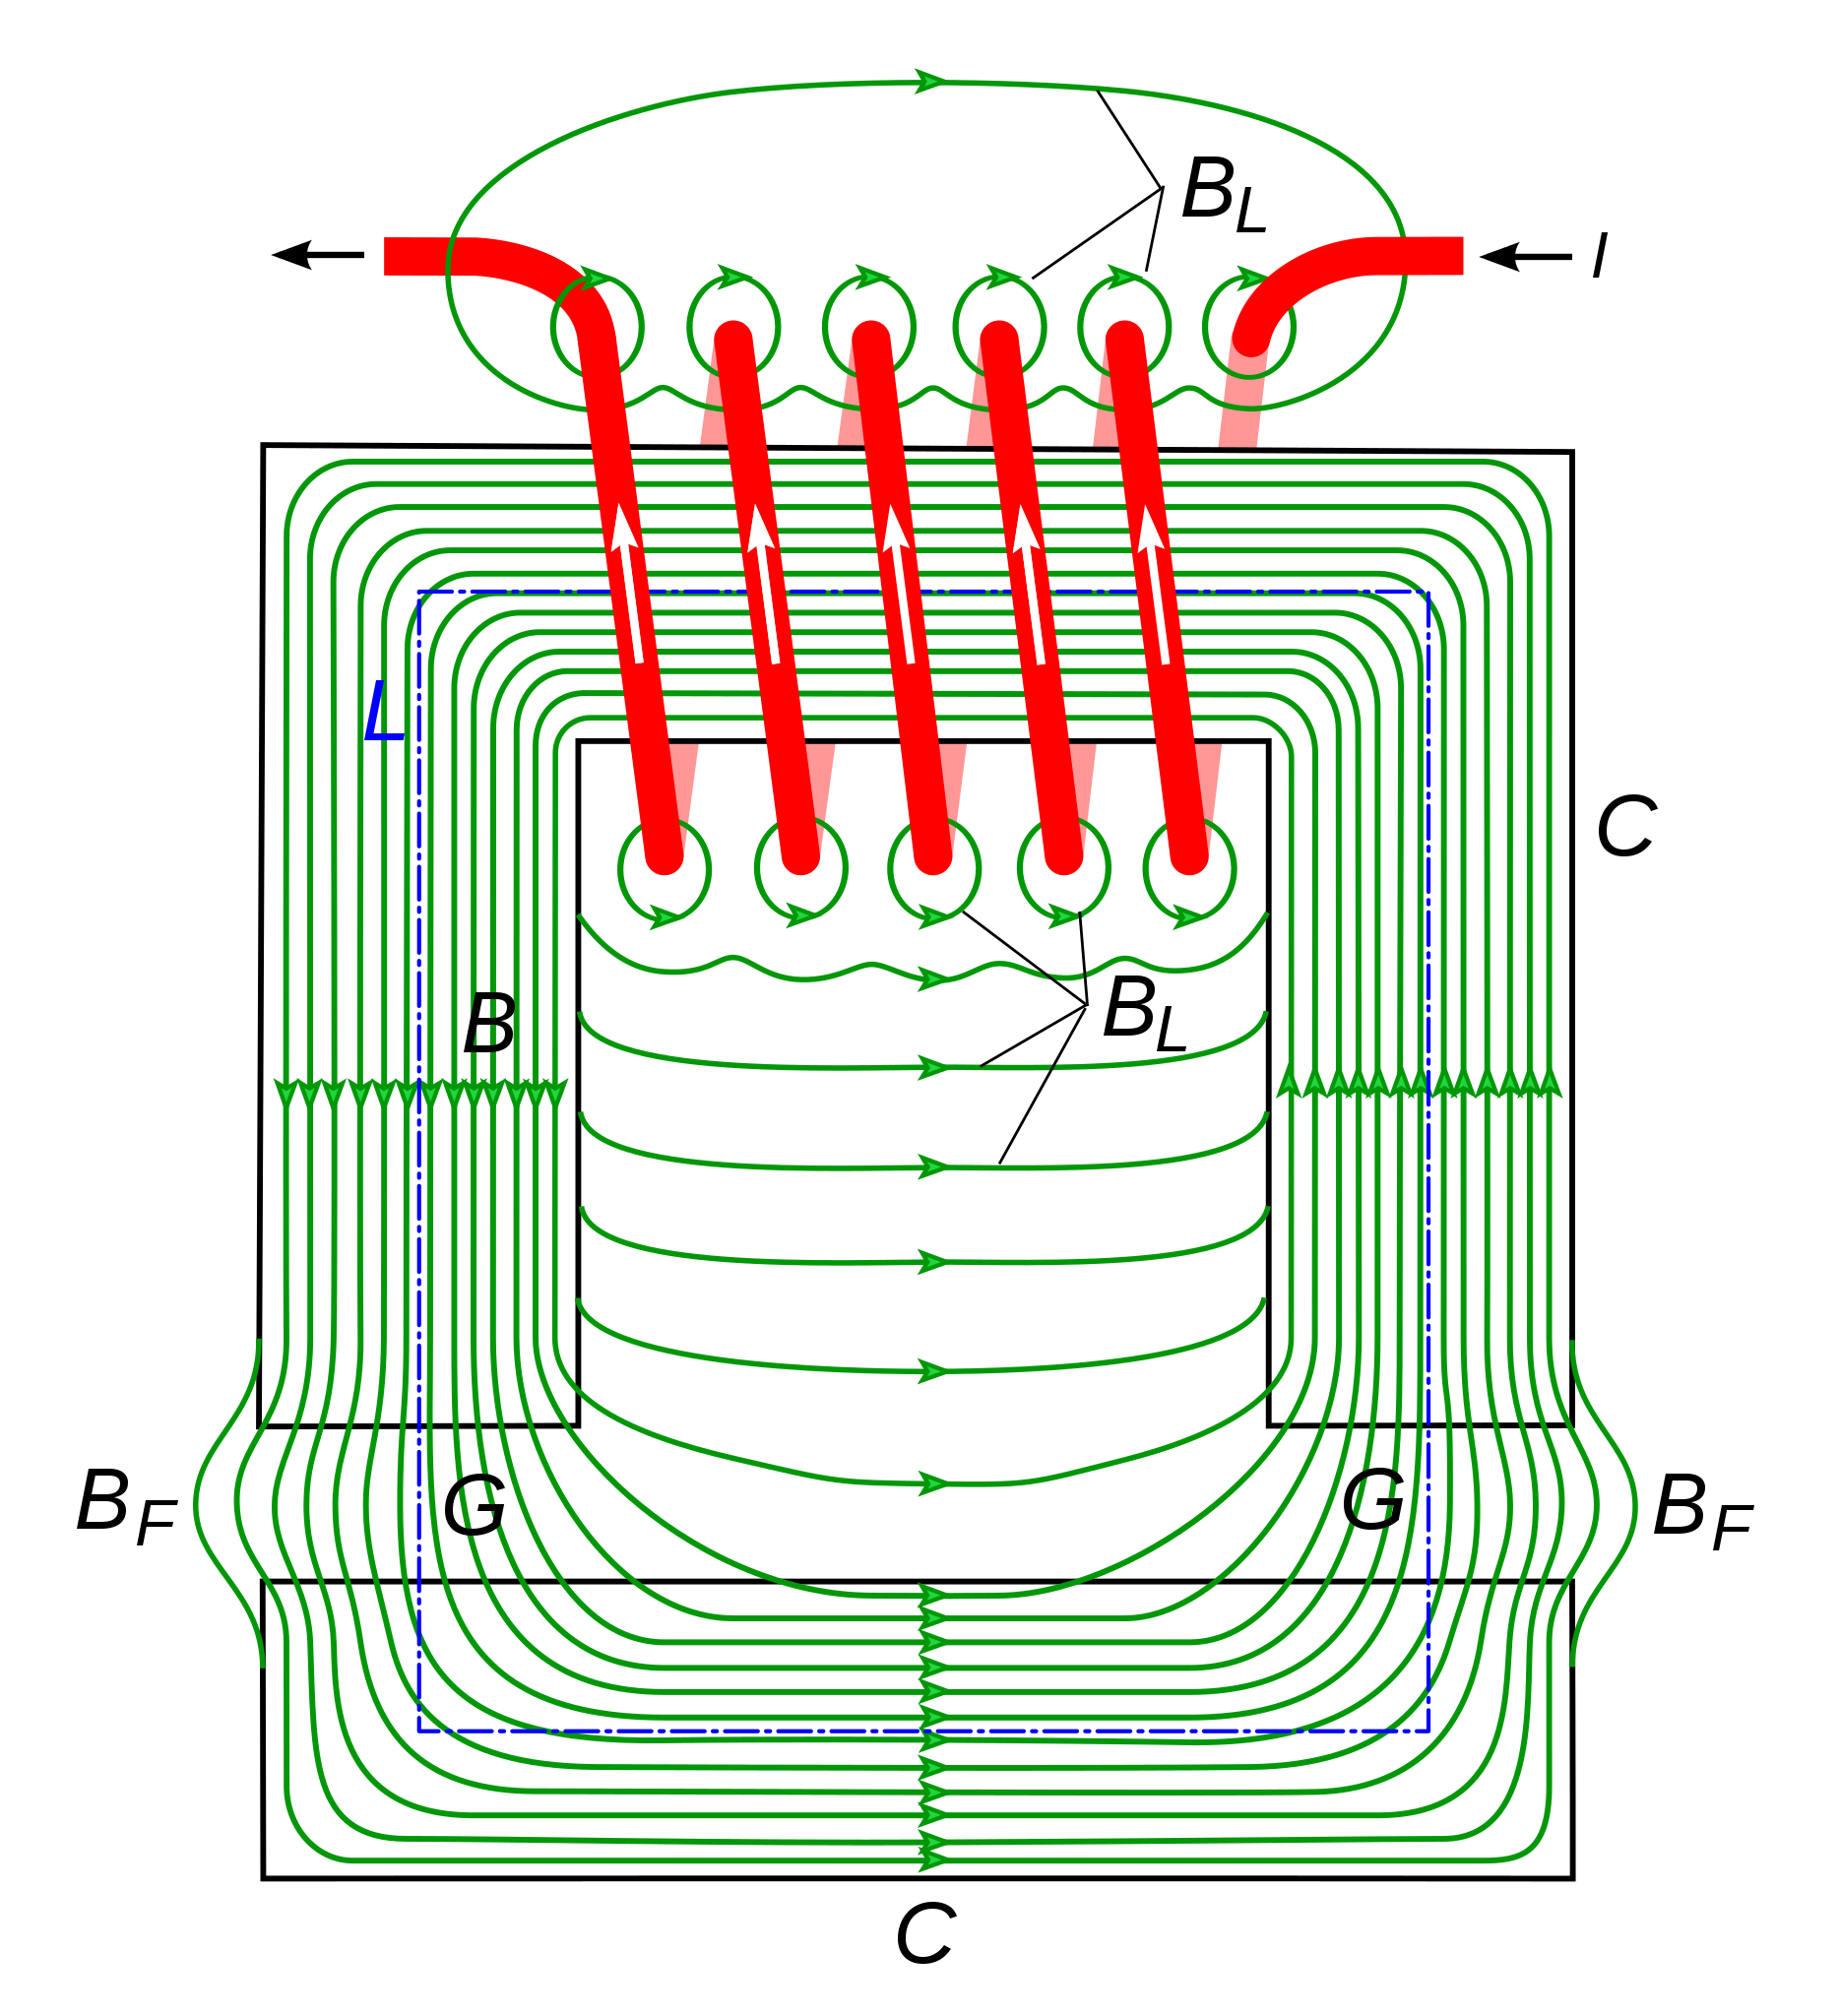
\includegraphics[width=0.7\columnwidth]{Electromagnet_with_gap.svg.png}
  \label{fig:chap:embasamento:6}
  \caption{Solenoide inserindo um campo magnético no núcleo, \cite{web:wikipedia:electromagnet}}
\end{figure}

Finalizamos então recordando a modelagem matemática desenvolvida ao longo do
curso de \cite{book:fitzgerald}, onde abstraímos a complexidade da modelagem de campos
por meio do conceito de Força Magneto-motriz e Relutância, trabalhando com fluxos e
comprimentos médios para a análise dos dispositivos.

\chapter{Motores}\label{chap:Motores}
Este capítulo discute a aplicação de eletroímãs no contexto de motores.

\bibliography{refs}

\end{document}
